% Rangefinding

\chapter{Rangefinding} % Main chapter title

\label{Rangefinding}

%----------------------------------------------------------------------------------------

This chapter covers the rangefinding subsystem, the subset of the project which determines the distances (ranges) between two sensors. The ranges are later fed into the position calculation subsystem, which determines the positions of the sensors in 3D space.

This chapter covers three main topics:
\begin{enumerate}
	\item A description of what the rangefinding system does and the devices it is made of.
	\item The math behind calculating the distance between two sensors.
	\item A description of the networking protocol developed for this project.
\end{enumerate}

\section{The System}
\begin{figure}
	\centering
	\tikzstyle{vertex}=[circle, draw]
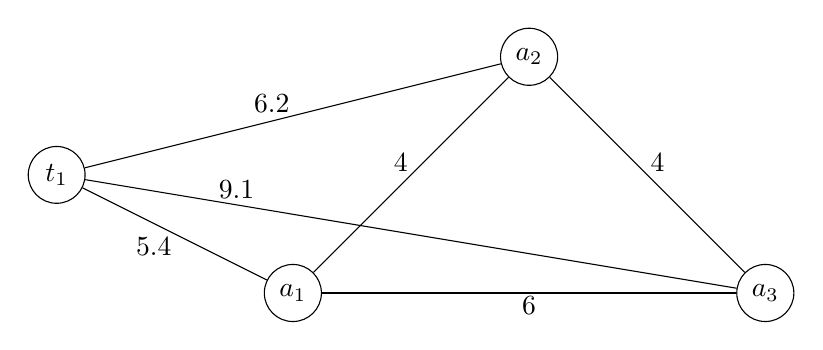
\begin{tikzpicture}[transform shape]
\node[vertex](a1) at (0, 0) {$ a_1 $};
\node[vertex](a2) at (3, 3) {$ a_2 $};
\node[vertex](a3) at (6, 0) {$ a_3 $};
\node[vertex](t1) at (-3,1.5) {$ t_1 $};

\begin{scope}[every path/.style={-}, every node/.style={inner sep=1pt}]
       \draw (a1) -- node [anchor=south east] {$4$} (a2);
       \draw (a2) -- node [anchor=south west] {$4$} (a3);
       \draw (a1) -- node [anchor=north] {$6$} (a3);
       \draw (t1) -- node [anchor=north east] {$5.4$} (a1);
       \draw (t1) -- node [anchor=south east] {$6.2$} (a2);
       \draw (t1) -- node [pos=0.2, anchor=south west] {$9.1$} (a3);
\end{scope} 
\end{tikzpicture}
	\decoRule
	\caption{An example network, showing 1 tag $t_1$ and 3 anchors $a_i$ and the reported distances between them.}
	\label{fig:ExampleNetwork}
\end{figure}

The rangefinding subsystem is comprised of \textbf{nodes} in a network, each of which is capable of sending and receiving wireless signals.

Each node is either an \textbf{anchor} or a \textbf{tag}. Both tags and anchors use essentially the same hardware and code, but anchors are assumed to be stationary while tags are mobile. Stationary nodes are required so as to provide a consistent frame of reference for other nodes when calculating positions later on. More information on this can be found in Section~\ref{FrameOfReference}.

The rangefinding subsystem's purpose is to determine the distances between every pair of nodes in the network. With this data, the position calculation subsystem can then determine the positions of every anchor and tag in 3D space. An example 2D rangefinding network is shown in Figure~\ref{fig:ExampleNetwork}.

\section{Rangefinding}
Rangefinding is the act of determining the distance between two objects. Rangefinding is done wirelessly in this project. The foundation of the technique is the idea that if the times at which a signal is sent and received between two nodes are precisely noted, then -- since light travels at a fixed speed -- we can determine the distance the signal traveled, which is the distance between the nodes. 

The nodes broadcast to every other node in the network whenever they transmit. A range calculation can be made whenever a response is received. Note that the range is calculated locally on each object, meaning a pair of nodes can believe they are different distances away from each other due to errors in the calculation of the range. Normally the ranges will be very close to each other, however.

The algorithm the network follows is: 
\begin{enumerate}
	\item Each node broadcasts a message to every other node, and every node responds. 
	\item The time it took for the message to travel from one node to another and then back (minus the time spent processing the received messages on the microcontroller) is calculated.
	\item Using the speed of light the distance between the nodes is calculated. 
\end{enumerate}

This method of calculating ranges is known as \textbf{time-of-flight} (TOF).

Each node is comprised of a Decawave DWM1000 ultra-wideband transceiver, which is what sends and the receives the rangefinding signals, and an Arduino microcontroller which actually calculates the ranges from timestamps obtained from the DWM1000. More information on the hardware can be found in Chapter~\ref{RangefindingHardware}.

\section{Time-of-Flight}
This section briefly covers the math behind time-of-flight range calculations. For more in-depth information, Decawave has a comprehensive write-up of the different ways wireless ranging can be performed as well as an error analysis \cite{DW1000UserManual}.

\subsection{Propagation Time}
The goal behind time-of-flight is to measure the propagation time of a signal, $T_{prop}$. Once we obtain this, it is a simple measure to calculate the distance $d$ between the two nodes using the speed of light, $c$, with the following formula:

\[
	d = c T_{prop}
\] 

\subsection{Single-sided Two-Way Ranging}
\begin{figure}
	\centering
	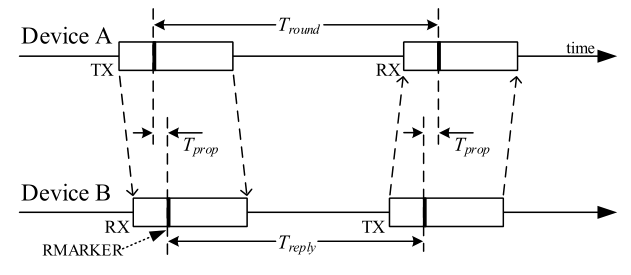
\includegraphics[width=\linewidth]{Figures/BasicRanging.png}
	\decoRule
	\caption{Single-sided two-way ranging \cite{DW1000UserManual}.}
	\label{fig:BasicRanging}
\end{figure}

In the case where there are two nodes communicating with each other, \parencite{DW1000UserManual} states that one can calculate the time it takes a signal to propagate between them, $T_{prop}$, as:

\[
	T_{prop} = \frac{T_{round} - T_{reply}}{2}
\]

where $T_{round}$ and $T_{process}$ are the total durations between receiving and transmitting messages as can be seen in Figure~\ref{fig:BasicRanging}.

\subsection{Double-sided Two-way Ranging}
\label{DSTWR}

\begin{figure}
	\centering
	\includegraphics[width=\linewidth]{Figures/AsyncRanging.png}
	\decoRule
	\caption{Double-sided two-way ranging with three messages \cite{DW1000UserManual}.}
	\label{fig:AsyncRanging}
\end{figure}

Because the clocks of two nodes may not pass time at the same rate (clock skew), the above equation will suffer from significant error. This is because processing times far dwarf the time it takes a signal to propagate. Decawave presents, without proof, the following equation for more accurate rangefinding \cite{DW1000UserManual}:

\[
	T_{prop} = \frac{T_{round1}  T_{round2} - T_{reply1} T_{reply2}}{T_{round1} + T_{round2} + T_{reply1} + T_{reply2}}
\]

where $T_{round1}$, $T_{round2}$, $T_{reply1}$, $T_{reply2}$ are the durations between sending and receiving messages as seen in Figure~\ref{fig:AsyncRanging}. An independently derived proof of this equation can be found in Appendix~\ref{AsyncProof}.

Because the ranging has two rounds, after the initial calculation of range we can calculate a new range value for every single following transmission by re-using the last timestamps received for the beginning of the next round.

\section{Requirements}
The scope of the project is to handle precise rangefinding in a small enclosed space, like an apartment. The requirements for the rangefinding subsystem system were:
\begin{itemize}
	\item The system must be able to produce ranges accurate to within three meters or less that are not noisy (regular swings of $\pm$ one meter would be unacceptable). If they are not, the AR portion of the project will not be able to show accurate ranges and may be misleading.
	\item The system must calculate ranges at frequencies greater than 3Hz. Otherwise, moving objects will have their positions displayed inaccurately and the system would be misleading.
	\item The system must be able to rangefind within an area the size of a room (at least 5x5 meters). 
	\item The system must be able to handle lost transmissions in case of interference. 
\end{itemize}

\section{Networking Basics}
Each node in the network broadcasts in a round robin fashion, with a small break after every node has transmitted. As part of a transmitted message, a node transmits the timestamp marking when the message was sent, a list of the timestamps noting when it last received a communication the other nodes in the network, and a list of the last computed ranges to the other nodes. Every other node in the network will use the timestamps contained in the message to compute a new range to the transmitting. Thus, every node in the network receives complete range information for the whole network.

Every node in the network has a pre-determined ID, which is set when the Arduino is programmed. A single byte is used for this ID to save as much space as possible, though the code could easily be modified to support longer IDs if the devices were to be mass produced. As there are only 7 devices currently operational, our project only uses IDs 1 through 7, though the IDs do need not be consecutive. ID 255 is a special dummy value used in the code and should not be selected for use with an actual device.

Communications between the Arduino and the DWM1000 are handled through SPI. When the DWM1000 receives a message, it triggers an interrupt on the Arduino, which can then obtain the received data through SPI.

\section{Communications Timing}
\begin{figure}
	\centering
	\begin{tikzpicture}

\def \n {6}
\def \radius {3cm}
\def \margin {11} % margin in angles, depends on the radius

\begin{scope}[auto, every node/.style={draw,circle,minimum size=2em,inner sep=1},node distance=2cm]
\foreach \id [count=\s] in {1, 2, 5, 8, 10, 255}
{
  \node at ({360/\n * (\s - 1)}:\radius) {$\id$};
  \draw[->, >=latex] ({360/\n * (\s - 1)+\margin}:\radius) 
    arc ({360/\n * (\s - 1)+\margin}:{360/\n * (\s)-\margin}:\radius);
}
\end{scope}

\end{tikzpicture}
	\decoRule
	\caption{Transmission order of a network composed of five devices with IDs 1, 2, 5, 8, and 10. Note they transmit in order, and there is a dummy ID of 255 which serves as a marker for the end of the round.}
	\label{fig:TransmissionOrder}
\end{figure}

In order to maximize the operating frequency of the system and provide as smooth a visual experience as possible on the phone, the amount of time a node is not transmitting should be minimized. As part of this goal, it was decided that nodes should transmit in order of their ID in a round robin fashion. A round of transmissions are performed, each node transmitting once, and then the round repeats. When one node receives a transmission, it checks to see if it is its turn and then transmits as soon as it has processed the message.

This round robin ordering is implemented via an ordered array of IDs on each device. The array contains the ID of every node that has been detected transmitting. When a transmission is received, the network increments the index of the next expected device to transmit by 1. A device can tell whether it should transmit by checking to see if its ID is equal to the ID of the next expected node to transmit. 

The downside to this approach is that if any transmission were to be lost, for example by interference or electrical noise, the network would grind to a halt as it waits for a message that is never going to come. The project's solution to this is to include a timer that tracks a window in which a message is expected to be received. If a message is not received in this window, the device that was expected to transmit is assumed to have to failed to transmit and the next device takes their turn and transmits.

To help the network be more robust, for example if one node has a clock that runs faster than the others (making it think a transmission is late when it is not), the network assumes whatever device last transmitted was right in doing so, and sets the index of the next node to transmit in the ordered array as being one higher than it.

This approach also raises the question of how new nodes can join the network if a node is constantly transmitting. To solve this, a small delay is added at the end of each round. When a device wishes to enter the network, it waits for the end of a round, and then does a transmission in this pause between rounds. This transmission lets all devices know it is part of the network, and it is added to the ordered array of IDs. (The edge case of a device's transmission failing when it is trying to join the network was ignored due to time constraints, but it is easy to solve manually via a reset of the device in question.)

To implement this, this delay at the end of the round is implemented by adding a dummy node with the ID of 255 (the highest ID possible with one byte) to the network. The nodes will wait for a transmission from it at the end of each round, but it will never come, at which point the round starts over with the lowest ID transmitting. An example ordering can be found in Figure~\ref{fig:TransmissionOrder}.

Code for this logic can be found in the \code{loop} function of the Arduino code. See Appendix~\ref{SourceCode}.

\section{Range Information Protocol}
\begin{figure}
	\centering
	\usetikzlibrary{calc,positioning,shapes,decorations.pathreplacing}

% the styles for short and long nodes
\tikzset{
short/.style={draw,rectangle,minimum height=1.5cm,
  text width=7pt,align=center,fill=gray!30, text centered},
long/.style={short,text width=1.9cm}
}

% the short nodes \shnode{<label>}{<right of>}{<text>}
\def\shnode#1#2#3{%
  \node[short,right=of #1] (#2) {\rotatebox{270}{#3}}}

% the long nodes \lnode{<label>}{<right of>}
\def\lnode#1#2#3#4{%
  \node[long,right=of #1,label={below:#4}] (#2) {#3}}
  
 \def\idnode#1#2#3#4{%
  \node[short,right=of #1,label={below:#4},style={short,text width=1.1cm}] (#2) {#3}}

\noindent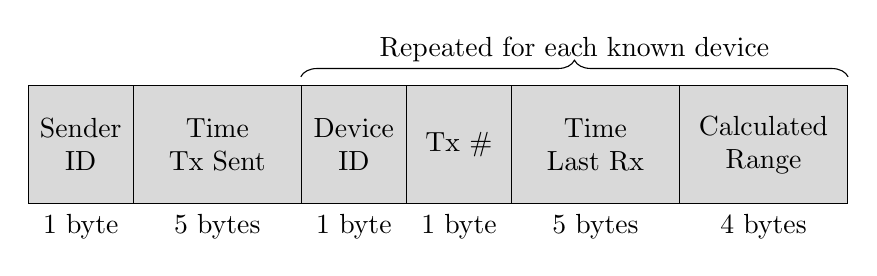
\begin{tikzpicture}[node distance=-\pgflinewidth]

\node[short,label={below:1 byte},style={short,text width=1.1cm}] (a) {Sender ID};
\lnode{a}{b}{Time Tx Sent}{5 bytes};
\idnode{b}{c}{Device ID}{1 byte};
\idnode{c}{d}{Tx \#}{1 byte};
\lnode{d}{e}{Time Last Rx}{5 bytes};
\lnode{e}{f}{Calculated Range}{4 bytes};

\draw[decorate,decoration={brace,raise=3pt,amplitude=0.6em}] (c.north west) -- node[above=5pt] {Repeated for each known device} (f.north east);

\end{tikzpicture}
	\decoRule
	\caption{Data packet diagram for the rangefinding network.}
	\label{fig:NetworkPacket}
\end{figure}

Every transmission made by a node contains timestamps so that receiving nodes can calculate how far away they are from the sending node.

The protocol for a transmission from a node is as follows:

\begin{itemize}
	\item 1 byte for the ID of the transmitting node. The ID cannot not be 255.
	\item 5 bytes for the timestamp of the sending of the message. The DWM1000 uses 40 bits (5 bytes) for its timestamps and has picosecond order resolution. The Arduino internally represents these as 64-bit integers, but transmits them as 40 bit (5 byte) numbers.
	\item For each device the transmitting node has knowledge of:
	\begin{itemize}
		\item 1 byte for the ID of the device.
		\item 1 byte for a shared transmission counter. This counter is incremented by one whenever a message is received, and also incremented when one is sent. If a message is received or sent and the transmission counter on the device does not match the counter in the message, a transmission was lost. The message is thrown away and the transmission counter set to 0 to let the other device know there was an error on the next transmission.
		\item 5 bytes for timestamp of last received message from the device.
		\item 4 bytes for last calculated range to that device. Note that the two devices will each calculate slightly different ranges to each other.
	\end{itemize} 
\end{itemize}

Ranges are calculated with the timestamps via the double-sided two-way ranging formula in Section~\ref{DSTWR}. The code in question can be found in the \code{parseReceived} function in the Arduino source code. See Appendix \ref{SourceCode}.

\section{Summary}
This section covered how a rangefinding network can be constructed, the higher-level aspects of the rangefinding system used in this project, including how ranges are calculated, and the networking protocol used.

Transmissions are done in a round-robin fashion, and every transmission includes timestamps so the receiving device can calculate a range. Performance metrics of the system are enumerated in Chapter~\ref{RangefindingHardware}.
